\documentclass[a4paper]{article}

\usepackage[a4paper,hmargin=2.8cm,vmargin=2.0cm,includeheadfoot]{geometry}
\usepackage{textpos}
\usepackage{tabularx,longtable,multirow,subfigure,caption}%hangcaption
\usepackage{fancyhdr} % page layout
\usepackage{url} % URLs
\usepackage[english]{babel}
%\usepackage{afterpage}
\usepackage{amsmath}
\usepackage{amssymb}
\usepackage{systeme}
\usepackage{graphicx}
\usepackage{dsfont}
\usepackage{epstopdf} % automatically replace .eps with .pdf in graphics
%\usepackage{backref} % needed for citations
\usepackage{array}
\usepackage{latexsym}
\usepackage{lipsum}
\usepackage{tikz}
\usepackage{xcolor}
\usepackage{tabularx}
\usepackage{makecell}
\usetikzlibrary{angles, arrows.meta, quotes}
\usepackage[pdftex,hypertexnames=false,colorlinks]{hyperref} % provide links in pdf

\usepackage[skip=10pt plus1pt, indent=40pt]{parskip}

\hypersetup{pdftitle={},
  pdfsubject={}, 
  pdfauthor={},
  pdfkeywords={}, 
  pdfstartview=FitH,
  pdfpagemode={UseOutlines},% None, FullScreen, UseOutlines
  bookmarksnumbered=true, bookmarksopen=true, colorlinks,
    citecolor=black,%
    filecolor=black,%
    linkcolor=black,
    linkbordercolor=blue,%
    urlcolor=blue}

\usepackage[all]{hypcap}


%\usepackage{color}
%\usepackage[tight,ugly]{units}
%\usepackage{float}
%\usepackage{tcolorbox}
%\usepackage[colorinlistoftodos]{todonotes}
% \usepackage{ntheorem}
% \theoremstyle{break}
% \newtheorem{lemma}{Lemma}
% \newtheorem{theorem}{Theorem}
% \newtheorem{remark}{Remark}
% \newtheorem{definition}{Definition}
% \newtheorem{proof}{Proof}


%%% Default fonts
\renewcommand*{\rmdefault}{bch}
\renewcommand*{\ttdefault}{cmtt}



%%% Default settings (page layout)
\setlength{\parindent}{0em}  % indentation of paragraph

\setlength{\headheight}{14.5pt}
%\pagestyle{fancy}
%\renewcommand{\chaptermark}[1]{\markboth{\chaptername\ \thechapter.\ #1}{}} 

%\fancyfoot[ER,OL]{\sffamily\textbf{\thepage}}%Page no. in the left on odd pages and on right on even pages
%\fancyfoot[OC,EC]{\sffamily }
%\renewcommand{\headrulewidth}{0.1pt}
%\renewcommand{\footrulewidth}{0.1pt}
\captionsetup{margin=10pt,font=small,labelfont=bf}



% %--- chapter heading

\def\@makessectionhead#1{%
  \vspace*{10\p@}%
  {\parindent \z@ \raggedright \sffamily
    \interlinepenalty\@M
    \Huge\bfseries \thesection \space\space #1\par\nobreak
    \vskip 30\p@
  }}

% %---chapter heading for \chapter*  
\def\@makeschapterhead#1{%
  \vspace*{10\p@}%
  {\parindent \z@ \raggedright
    \sffamily
    \interlinepenalty\@M
    \Huge \bfseries  #1\par\nobreak
    \vskip 30\p@
  }}

\allowdisplaybreaks
%\usepackage[pages=all, color=black, position={current page.south}, placement=bottom, scale=1, opacity=1, vshift=5mm]{background}

% AMS Packages
\usepackage{amsmath}
\usepackage{amsthm}
\usepackage{amssymb}

% Unicode
\usepackage[utf8]{inputenc}
\usepackage{hyperref}
\hypersetup{
	unicode,
%	colorlinks,
%	breaklinks,
%	urlcolor=cyan, 
%	linkcolor=blue, 
	pdfauthor={Author One, Author Two, Author Three},
	pdftitle={A simple article template},
	pdfsubject={A simple article template},
	pdfkeywords={article, template, simple},
	pdfproducer={LaTeX},
	pdfcreator={pdflatex}
}


% Natbib
\usepackage[sort&compress,numbers,square]{natbib}
\bibliographystyle{unsrt}

\usepackage{graphicx, color}
\graphicspath{{figures/}}

\usepackage{mathrsfs} % for \mathscr command

\usepackage{orcidlink}

\usepackage{listings}
\newcommand{\R}[0]{\mathds{R}} % real numbers
\newcommand{\Z}[0]{\mathds{Z}} % integers
\newcommand{\N}[0]{\mathds{N}} % natural numbers
\newcommand{\C}[0]{\mathds{C}} % complex numbers
\renewcommand{\vec}[1]{{\boldsymbol{{#1}}}} % vector
\newcommand{\mat}[1]{{\boldsymbol{{#1}}}} % matrix
\lstset{ %
    basicstyle=\ttfamily\footnotesize,
    commentstyle=\color{ForestGreen},
    frame=single,
    keywordstyle=\color{black},
    language=Bash,
    showstringspaces=false,
    %morekeywords={blue},
    morestring=[s][\color{Gray}]{<}{>},
    morestring=[s][\color{OrangeRed}]{\ -}{\ },
    morestring=[s][\color{OrangeRed}]{*}{\ },
    morestring=[s][\color{OrangeRed}]{|}{\ },
    morestring=[s][\color{OrangeRed}]{\&}{\ },
}
\renewcommand{\lstlistingname}{Command}
%----------------------------------------------------------------------------------------


% Author info
\title{Report on: Molecular dynamics simulations of the stabilization of pea diamine oxydase structure with trehalose}
\author{Pau Domínguez-Sorribas$^1$\thanks{Author One developed his work during his BSc final project} \and Jordi Villà-Freixa$^{1,2}$\orcidlink{0000-0002-6359-3929}}

\date{
	$^1$Research Group on Bioinformatics and Bioimaging, Department of Biosciences, Universitat de Vic - Universitat Central de Catalunya (UVic-UCC), Vic, Spain \\ \texttt{\{pau.dominguez, jordi.villa\}@uvic.cat}\\
	$^2$Institut de Recerca i Innovació de la Catalunya Central (IRIS-CC), Vic, Spain. \\[2ex]%
	\today
}

\begin{document}
	\maketitle
	
	\begin{abstract}
		
		This report delves into the molecular dynamics (MD) simulations of pea diamine oxidase (DAO) in the presence and absence of trehalose molecules, using with the AMBER MD software suite. The primary aim is to investigate the stabilizing effects of trehalose on DAO, an enzyme crucial for the metabolism of biogenic amines. DAO simulations are conducted in a truncated octahedral box with periodic boundary conditions to emulate an infinite system, enhancing the realism of the molecular environment. 
		
		\noindent\textbf{Keywords:} Diamine oxydase, protein stability, trehalose, molecular dynamics, AMBER
	\end{abstract}

	\tableofcontents

		\section{Introduction}
	\label{sec:intro}
	
	It is well recognized that saccharides have exceptional properties in helping biomolecules such as proteins preserve their native structures under harsh conditions, e.g., high or low temperatures, and dehydration\cite{shao_trehalose_2019,crowe_lessons_2002,cao_effect_2008}. Among naturally available saccharides, trehalose, a nonreducing homo-disaccharide in which two D-glucopyranose units are linked together by an $\alpha$-1,1-glycosidic linkage (Figure 1 (a)) is probably the best biomolecule stabilizer\cite{hedoux_thermostabilization_2009,shao_trehalose_2019,jain_role_2008,jain_effect_2009,kaushik_why_2003}. As a result, trehalose is widely used as additive for long-term preservation of therapeutic proteins, foods, and cosmetics industries\cite{carpenter_rational_1997,higashiyama_novel_2002,arakawa_factors_2001,shao_trehalose_2019}.

	\subsection{Diamine oxidase}

In this project, we focus on a probiotic developed by a partner biotech company. This probiotic, among other constituents, contains diamine oxidase (DAO), a copper amine oxidase (CAO) which, due to its instability, gets rapidly degraded in the final product. A representation of DAO structure, as obtained from PDB code 1KSI\cite{1ksi}, is shown in Figure \ref{fig:structure}.

\begin{figure}[h]
    \centering
    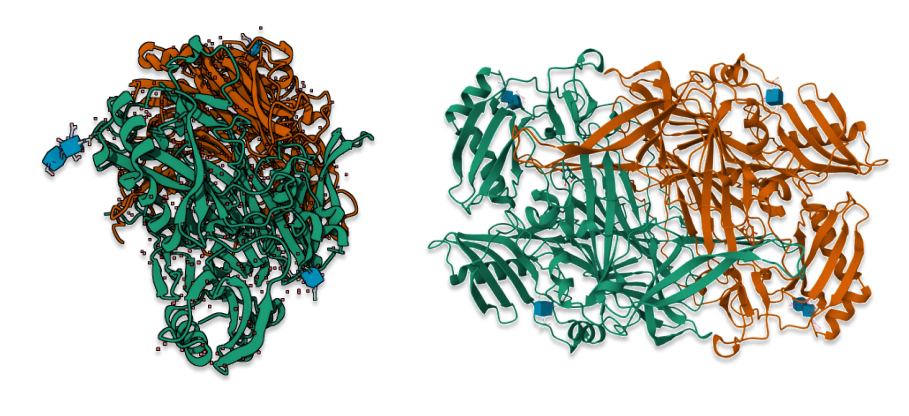
\includegraphics[width =\hsize]{1KSI}
    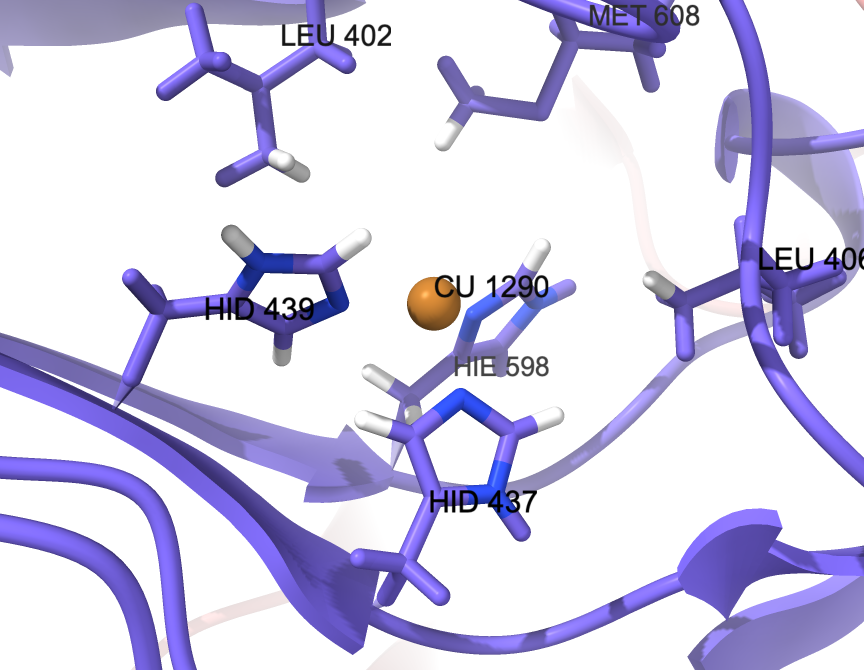
\includegraphics[width =0.5\hsize]{activesite_daoamber}
    \caption{a) Quaternary structure of DAO, indicating $\alpha$ helices (yellow), $\beta$ strands (green) and loops (no color). Notice the position of TPQ (in red). b) Detail of the active site, with the coordination of the Cu$^{+2}$ ion in chain A. Note that the numbering corresponds to that in the AMBER calculation (5 residues are msising in the N-terminal for each of the two units of the biologically active DAO. Obtained with ChimeraX; PDB code: 1KSI.}
\label{fig:structure}
\end{figure}

Figure 




Copper amine oxidases (CAOs) have been extensively studied across various domains of life\cite{mcgrath_structure_2009}, revealing a common architectural motif despite differences in origin. Structures from bacteria (Escherichia coli; Arthrobacter globiformis), yeast (Hansenula polymorpha; Pichia pastoris), plants (Pisum sativum), and mammals (Homo sapiens; Bos taurus) share homodimeric arrangements\cite{floris_copper_2009}, each subunit typically comprising around 700 amino acid residues (Figure \ref{fig:seq}). The pioneering E. coli enzyme's structure\cite{parsons_crystal_1995} resembled a mushroom, with the stalk formed by D1 domains and the cap by D2, D3, and D4 domains of each subunit. 

\subsubsection{Cofactors and postranslational modifications}

A part from Cu$^{+2}$ and Mn$^{+2}$  ions, this protein has two important molecules attached to its structure (Figure:\ref{fig:NAGTPQ}). First one is the modified residue topaquinone (TPQ) and the second one would be NAG (N-Acetyl-D-Glucosamyine) that is presented in two forms, as a ligand where only one molecule of NAG is linked to the protein by an asparagine, and as polymer where two molecules of NAG joined together are linked to an asparagine in the protein.

TPQ or topaquinone is the modified residue we find in our enzyme DAO. It consists on a redox cofactor derived from tyrosine residue where two additional oxygen atoms have been attached. Its biogenesis proceeds by a sel-processing pathway which requires only the protein, copper and molecular oxygen. Not only is found in plants like in our case but in bacteria, mammals or fungi.
As a result of previous studies, specifically those that helped out to crystallographically establish DAO structure, we know that TPQ presents a conformational flexibility which is the capacity of side chains and polypeptide backbone fragments to take on various conformations while preserving the original protein structure \cite{1ksi}.


NAG generally is refered to 2-acetoamido-2deoxy-beta-D-glucopyranose or N-Acetyl-D-Glucosamine which is a ligand attached to the protein. It is also a N-Glycan since is covalently attached to the protein at asparagine (Asn) rsidues by an N-glycosidic bond. N-Glycans affect to the protein properties, including their conformation, solubility, activity... Which are factors to must have into account to study a protein.
It derives from a glucose monosaccharide forming an amide between glucosamine and acetic acid.
In our case we have six different NAGs in four different positions: 2 of them are simple N-Glcyans covalently attached to the protein at asparagine, but only one NAG linked to that asparagine; the other four consist in two carbohydrate polymers also attached to an asparagine: Each polymer consists in two NAGs linked between them and then attached to an asparagine\cite{Tekin2023}.

\begin{figure}[h]
    \centering
    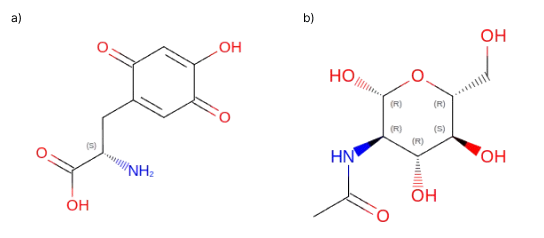
\includegraphics[width = 0.8\hsize]{./figures/nagtpq}
    \caption{Chemical structure of diamine oxidase cofactors: TPQ (a) and NAG (b)configuration image obtained by PDBe code= 1KSI: NAG, TPQ}
    \label{fig:NAGTPQ}
\end{figure}

Comparing various studies which has N-linked glycans, we can asume that our NAGs exercise the same function related with proper folding of the protein and their structure stabilization.

\begin{figure}[h]
    \centering
    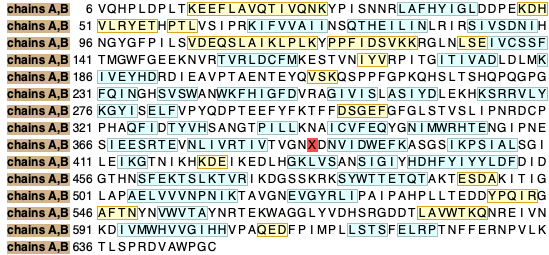
\includegraphics[width =\hsize]{seq}
    \caption{Primary structure of DAO, indicating $\alpha$ helices (yellow), $\beta$ strands (green) and loops (no color). Notice the position of TPQ (in red). Obtained from ChimeraX; PDB code: 1KSI.}
\label{fig:seq}
\end{figure}

Notably, the two active sites, situated in the D4 domains, house copper ions and the characteristic trihydroxyphenylalanine quinone (TPQ) cofactor. TPQ, crucial for enzyme function, forms post-translationally from a tyrosine residue in the presence of copper ions and molecular oxygen.

The enzymatic mechanism involves a ping-pong reaction, commencing with a reductive half where the substrate amine reacts with TPQ to form a Schiff base. This step is followed by an oxidative half, resulting in the release of the aldehyde product and reoxidation of the enzyme facilitated by molecular oxygen. While structures from other organisms mirror the E. coli CAO, they typically lack the D1 or stalk domain. Despite these variations, the fundamental architecture and catalytic mechanism remain conserved, highlighting the evolutionary significance and functional conservation of CAOs across diverse biological systems

The diamine oxidase used in this probiotic comes from a plant which is an enzyme involved in the metabolism, oxidation, and inactivation of histamine and other polyamines; being the main reason why it is used in this product because intolerance to histamine or its non-regulation can lead to gut problems.

Referring to histamine, the low level concentration of intestinal histaminase (whose the main function is to oxidize histamine) in the human body, together with some food intake like chocolate, beer, red wine or fish can eventually cause histaminosis, which is a dysfunction associated with pseudo allergy phenomenon\cite{Jumarie2017} where an excess of histamine in blood is present. 
	


\subsection{Trehalose as a protein stabilizer}

Mycose, tremalose or better known as trehalose ($\alpha$,$\alpha$-trehalose) is a common dissacharide derived from glucose. It is formed by a 1,1-glycosidic bond between two $\alpha$-glucose (Figure \ref{fig:tre2D}).

\begin{figure}[h]
    \centering
    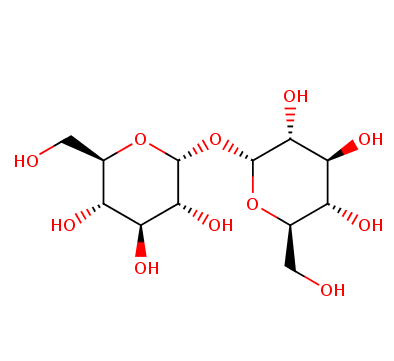
\includegraphics[trim= 10 60 10 90,clip,width = 0.4\hsize]{./figures/trehalosa}
    \caption{Chemical structure of trehalose}
    \label{fig:tre2D}
\end{figure}


Thanks to its chemical and biological properties it's expected to be a good stabilizer for our protein in the further simulations. It's been proved that some carbohydrates have the ability to stabilize proteins in several extreme conditions because of its resistance to hydrolysis, high temperatures or acidic conditions\cite{shao_trehalose_2019}.

Through hydrogen bonding, trehalose directly interacts with and influences the interactions between the other species by: Intermolecular hydrogen bonding interaction causing trehalose molecules to cluster; formation of hydrogen bonds between water and trehalose; influencing the strength of the water-water hydrogen bonding network without affecting protein-water hydrogen bonding and forming hydrogen bonds towards proteins while also replacing surrounding water molecules, reducing the possibility of hydrogen bonding from water to protein in accordance with the "water replacement" scenario.


	\subsection{Hypothesis and objectives}
	\label{sec:hypobj}
	
	Main hypothesis is that, in agreement with previous studies, trehalose follows a water replacement process around the protein structure to estabilize the latter. This in connected with a change in entropy in the water solvation, similar to what occurs in hydrophobic processes, where water is displaced from an interaction. This may mean that the effect of trehalose is not enthapically driven but entropically, and the presence of trehalose molecules around the protein limits the flexibility of the protein and makes it, thus, more reluctant to denaturalization processes. The fact that trehalose is the best saccaride to create such environment should be tested with other saccarides, and thus the inner features of trehalose that makes it especiffically relevant to enhance the protein structure may be revealed.

	Objectives:

	\begin{enumerate}
		\item Generate metrics for the stability of DAO surreounded by different solvent mixtures (pure water, water/trehalose mixtures, and water/other dissaccarides mixtures)
		\item Find ways to evaluate the enthalpy and entropy of the water desolvation processes in the mixtures simulations, and apply them to dissect the free energy of solvation in each case.
	\end{enumerate}
	
%%%%%%%%%%%%%%%%%%%%%%%%%%%%%%%%%%%%%%%%%%%
%%%%%%%%%%%%%%%%%%%%%%%%%%%%%%%%%%%%%%%%%%%
%%%%%%%%%%%%%%%%%%%%%%%%%%%%%%%%%%%%%%%%%%%
%%%%%%%%%%%%%%%%%%%%%%%%%%%%%%%%%%%%%%%%%%%
%%%%%%%%%%%%%%%%%%%%%%%%%%%%%%%%%%%%%%%%%%%
\section{Methodology}

All simulations have been done with Amber following the workflow in Figure \ref{fig:workflow}.  Protein structures where visualized with ChimeraX \cite{Chimerax} and trajectories analyzed with  VMD\cite{HUMP96} and cpptraj\cite{roe_ptraj_2013}, as well as xmgrace\cite{turner_xmgrace_2005} for plotting.

On AMBER calculations:
\begin{itemize}
    \item GAFF2 force field\cite{he_fast_2020} for TPQ
\end{itemize}


	\section{Results}
	\label{sec:results}


\subsection{Trehalose simulaltions results}

In order to firstly verify that trehalose behaves as a stable molecule in a water system with same parameterization as the final simulation of DAO with NAG, ions and trehalose; 5 different simulations of different concentration of trehalose molecules were run roughly 100 ns each. The results given from production process that are more important for us to analyze are the trajectory ones (\texttt{*.nc}) and the initial product topology file from each tleap. To visualize that trajectory with an RMSD (Root Mean Square Deviation) the tool cpptraj was used. 



Figure \ref{fig:rmsdtre} presents the Root Mean Square Deviation (RMSD) plots for five molecular dynamics (MD) simulations of trehalose molecules. Subfigures a, b, c, d, and e depict the RMSD trajectories for systems with 1, 2, 5, 10, and 25 trehalose molecules, respectively. All simulations were conducted for 100 ns, with the RMSD values stabilizing after an initial equilibration period. The plots indicate that each system maintained structural stability throughout the simulation duration, showcasing the consistent behavior of trehalose molecules in varying quantities under the simulated conditions. This stability is crucial for validating the reliability of the MD setup and a first indication of the appropriateness of the force field used to represent the disaccaride interactions.

\begin{figure}
    \centering
    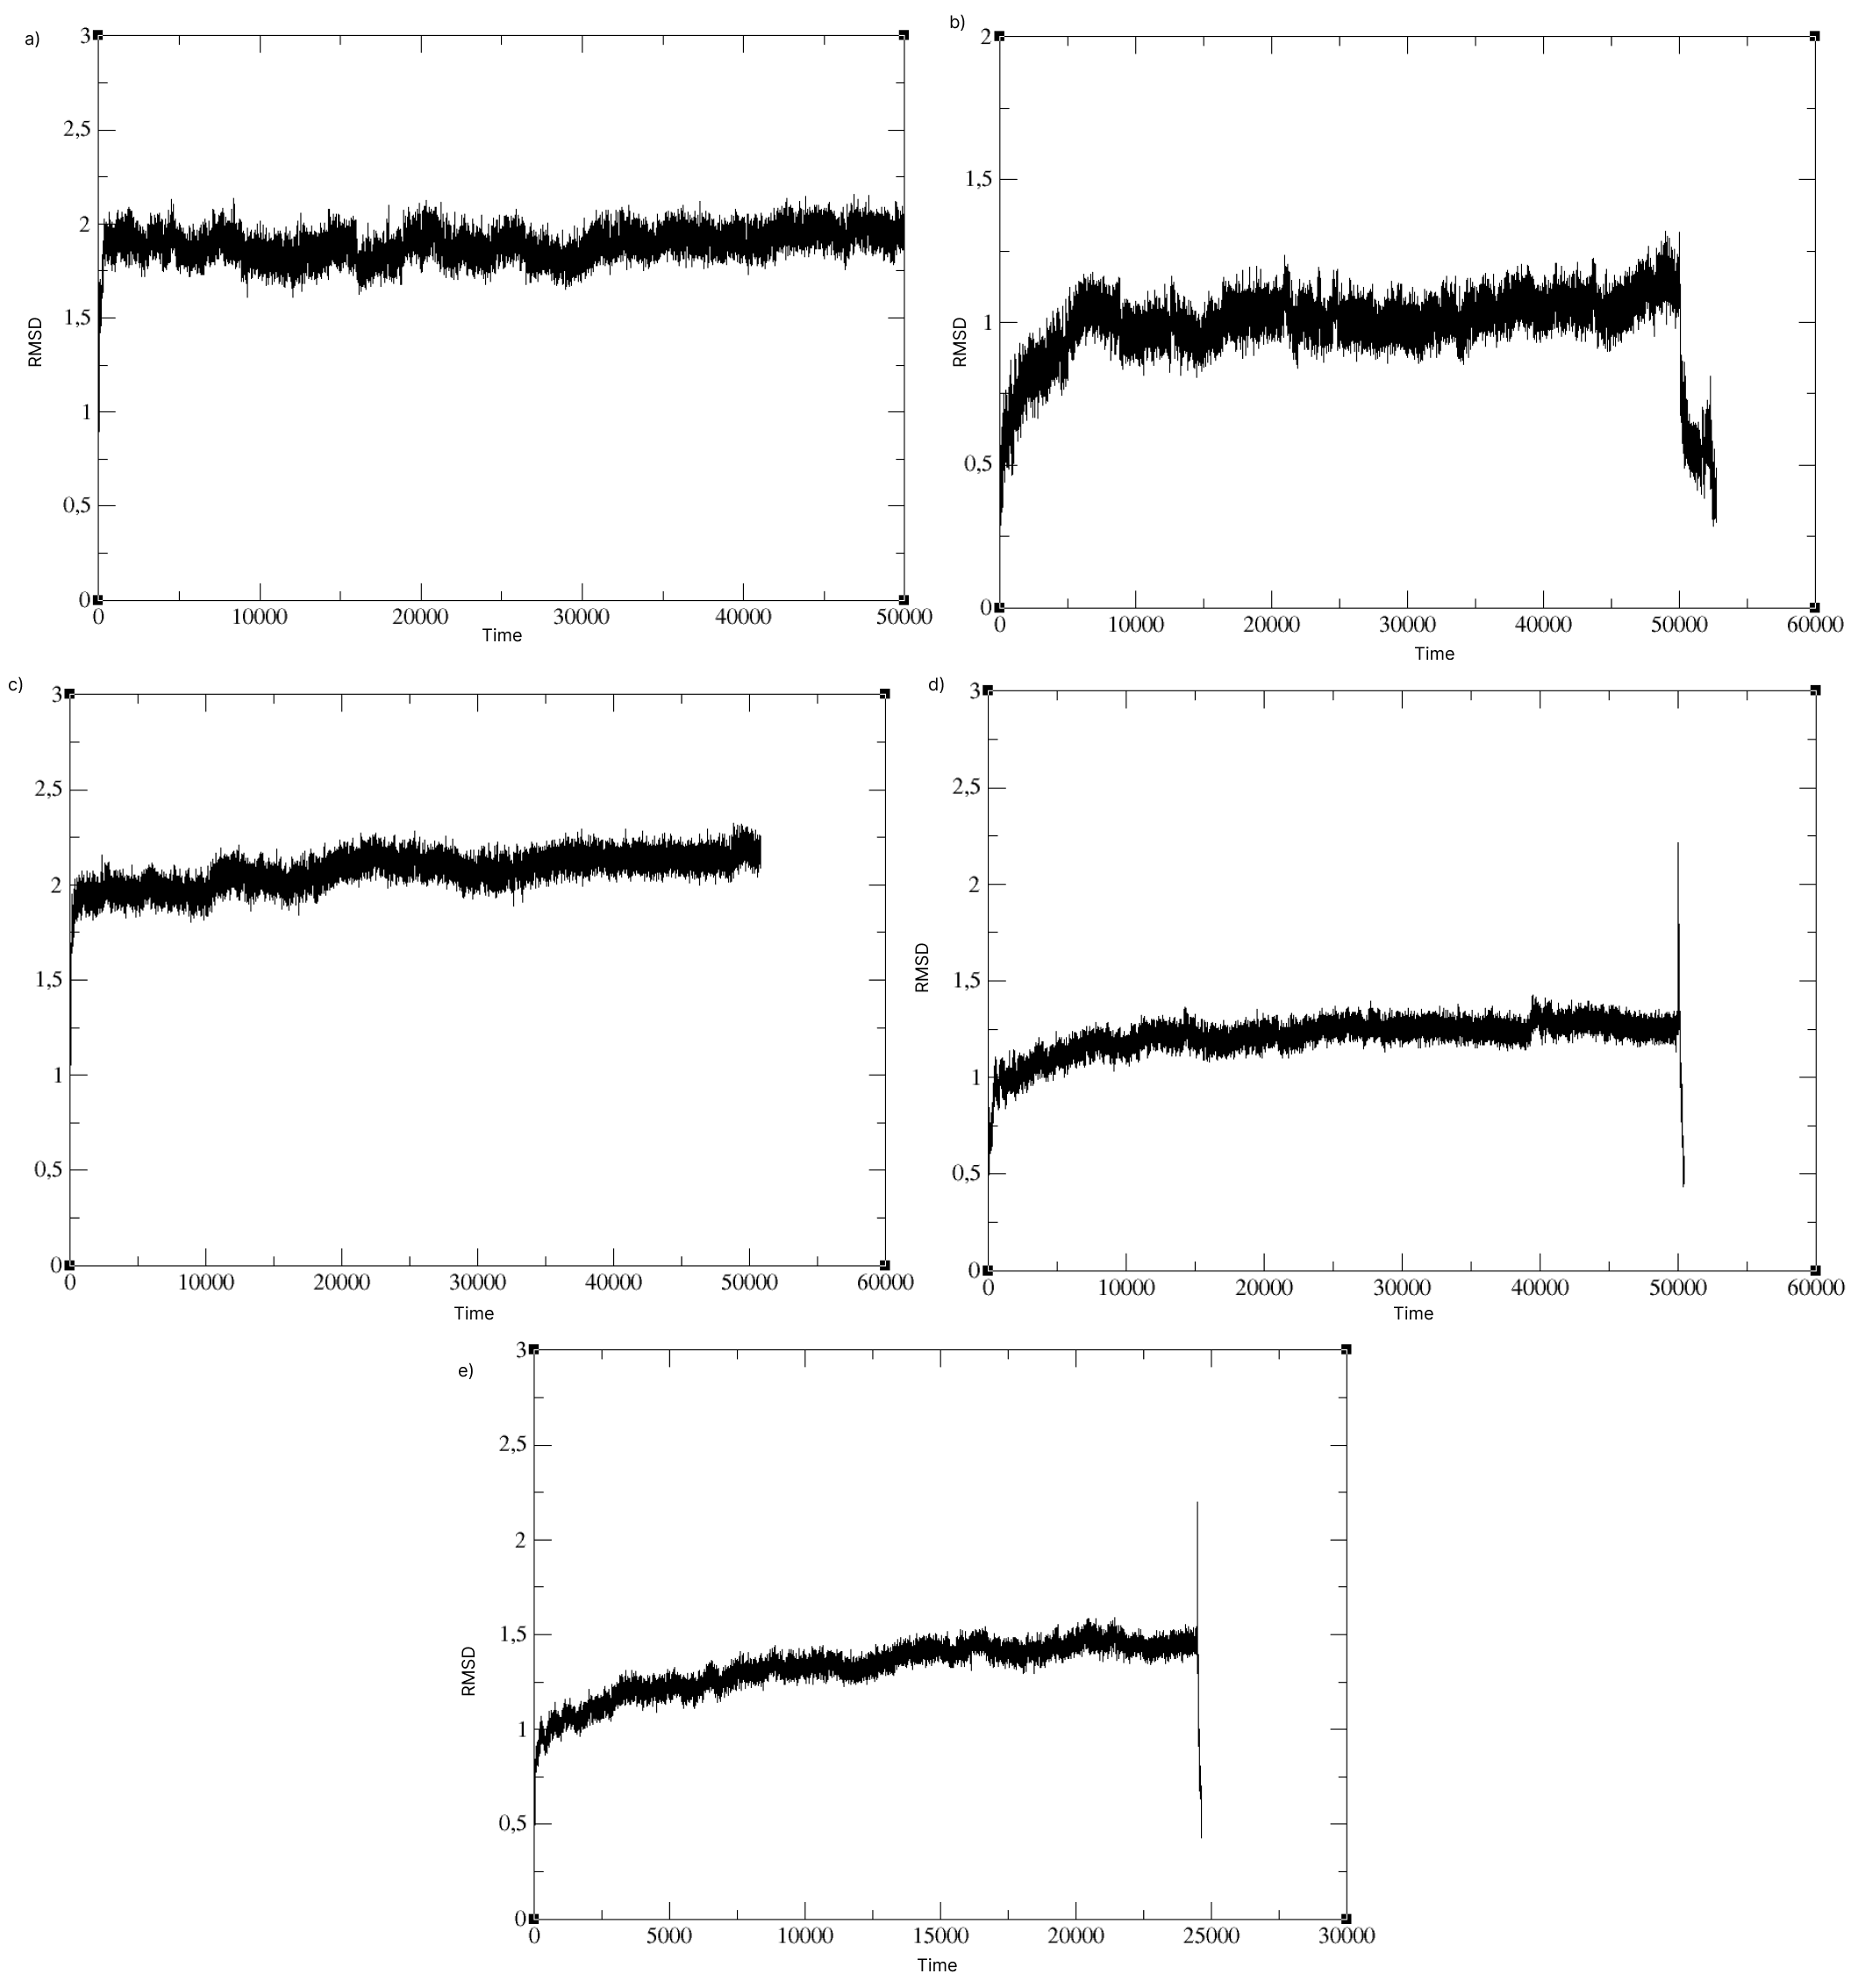
\includegraphics[width = 0.8\hsize]{rmsdtretot}
    \caption{Graphical representations of RMSD results from each of the trehalose simulations: a) 1 trehalose molecule, b) 2 trehalose molecules, c) 5 trehalose molecules, d) 10 trehalose molecules and e) 25 trehalose molecules.}
\label{fig:rmsdtre}
\end{figure}

\subsection{DAO without NAG, ions or trehalose in water system results}

After collecting all the data once the simulation was runned during 500 ns, it has to be prepared to be analyzed. Considering that each simulation result takes up a lot of space in the hard disk the the process must be carried out in an orderly and correct manner.
After trehalose results next results to be collected were those from DAO without NAG or trehalose simulation. Since the calculations took longer to be performed, the more runs were needed and therefore the size of each file. Due to this files size and the local computer used for this project which does not have a high storage capacity, the graphs created to visualize the results are from only some of the files (Figure \ref{fig:rmsdDAOnoNAG}). As it can be seen, even though the graphs are not made from all the files we can observe by the RMSD that the trehalose started to become unsettled. 



\begin{figure}[h]
    \centering
    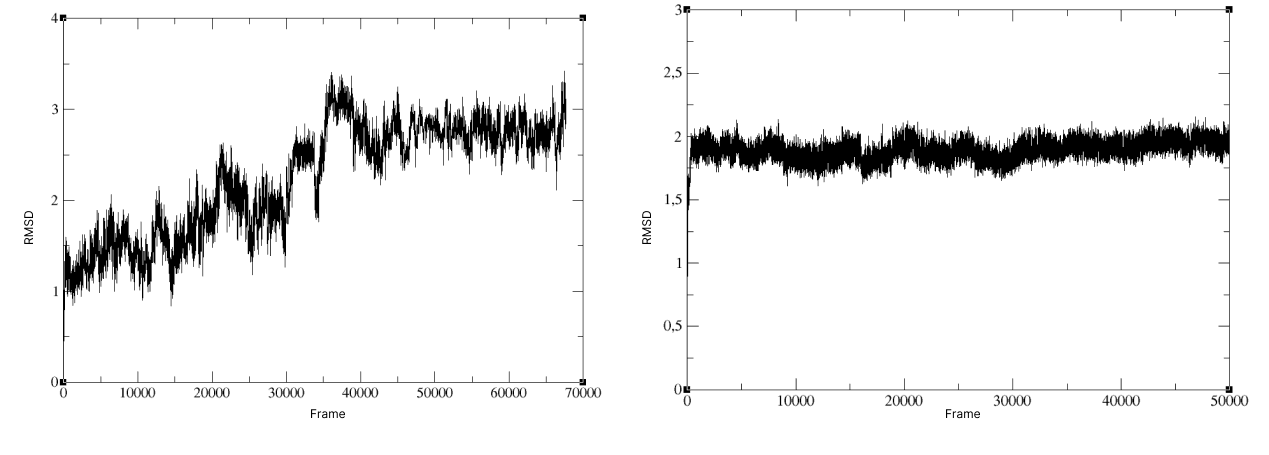
\includegraphics[width = 1\hsize]{./figures/rmsdmd1}
    \caption{Two RMSD graphs from the first four runs of the simulation (left image) and the first run of the simulation (right image) showing the measure of the average distance between the atoms}
    \label{fig:rmsdDAOnoNAG}
\end{figure}


\subsection{DAO with NAG and trehalose results}

The simulation which was going to be used, could not be realized. During the process of preparation of files everything was running as it was expected, except when the problems started once the tleap file was attempted to be run.
As the simulation could not be performed, there are no results to be analyzed and compared to previous ones.
	
\newpage
\section{References}
\bibliography{refs}
\newpage
%%%%%%%%%%%%%%%%%%%%%%%%%%%%%%%%%%%%
%%%%%%%%%%%%%%%%%%%%%%%%%%%%%%%%%%%%
%%%%%%%%%%%%%%%%%%%%%%%%%%%%%%%%%%%%
%%%%%%%%%%%%%%%%%%%%%%%%%%%%%%%%%%%%
%%%%%%%%%%%%%%%%%%%%%%%%%%%%%%%%%%%%
%%%%%%%%%%%%%%%%%%%%%%%%%%%%%%%%%%%%
%%%%%%%%%%%%%%%%%%%%%%%%%%%%%%%%%%%%
%%%%%%%%%%%%%%%%%%%%%%%%%%%%%%%%%%%%
%%%%%%%%%%%%%%%%%%%%%%%%%%%%%%%%%%%%
\appendix


\section{Supplementary material}

\setcounter{figure}{0}% Reset figure counter
\let\oldthefigure\thefigure% Capture figure numbering scheme
\renewcommand{\thefigure}{S\oldthefigure}% Prefix figure number with S

All details on the calculations are compiled in the GitHub repository \href{https://github.com/JordiVillaFreixa/Pau\_TFG\_DAO}{https://github.com/JordiVillaFreixa/Pau\_TFG\_DAO}.


\begin{figure}[h]
\centering
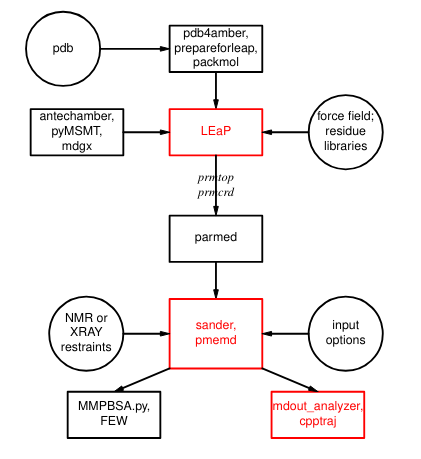
\includegraphics[width = 0.7\hsize]{workflow}
\caption{Basic workflow of a molecular dynamics simulation done with Amber (extracted from Amber 2023 Reference Manual)}
\label{fig:workflow}
\end{figure}

\subsection{Preprocessing files}

    
The "linkofinterest" is where it goes the copied link that refers to the files. Download command has to be runned multiple times, one for each file is precised.
After the download, is recommended to check and verify that we have the exact ones and the file is correctly structured. Analyzing 1KSI PDB file, the following message can be found: "NAG C 1 HAS WRONG CHIRALITY AT ATOM C1 NAG D 1 HAS WRONG CHIRALITY AT ATOM C2" 

Until the protein is analyzed it cannot be assured that it may affect in the future simulations, although it has been previously stated that N-glycans affect to the protein in several ways, so it is likely to have an effect in some way.

\subsection{Preparation of files}

Once all the needed files are downloaded in their respective structure, they have to be prepared for the use in Amber, because if left as they are, Amber is not going to recognize their structure and will not be useful. To start it will be prepared the main objective file of this study which is DAO. By running the simply command below, the file will be processed:

\begin{lstlisting}[language=Bash,caption={Preparing a pdb file to be used in \texttt{Amber}}]
    pdb4amber -i 1KSI.pdb -o DAO.pdb --reduce --dry
\end{lstlisting}


The command itself, what it does is to restructure the input PDB file into a new one that Amber can recognize. In addition, the "reduce" and "dry" words remove the crystallographic waters the file contains and adds hydrogen atoms in their optimal positions \cite{Amber23}.

Being the protein PDB file prepared, the following thing to do is prepare the cofactor files remaining. First file of the two to be prepared after the protein one is TPQ.cif, the modified residue in DAO. As a modified residue is not considered a standard residue that the program can recognize, so a new entry on the Amber library will be needed for Amber to recognize and process once the file is loaded for the final simulations.
The first thing TPQ.cif file needs, is to be processed by \href{https://ambermd.org/antechamber/ac.html}{Antechamber}, which is a set of auxiliary programs for molecular mechanic studies that solves the following problems during the MM calculations:
\begin{enumerate}
    \item Recognition of the atom type
    \item Recognition of bond type
    \item Judging the atomic equivalence
    \item Generation of residue topology file
    \item Finding of missing force field parameters
\end{enumerate}
To obtain an output file with atom types and partial charges an Antechamber command is going to be used. The command is as follows:

   
\begin{lstlisting}[language=Bash,caption={Antechamber for TPQ}]
    antechamber -fi ccif -i TPQ.cif -bk \
                TPQ -fo ac -o tpq.ac -c bcc -at amber
\end{lstlisting}

The usage of Antechamber may vary depending on the input file format, the output file format, charge method... So it depends on the parameterization one wants to do.
This command let the input file TPQ.cif be transformed into a new file containing now atom types and partial charges. At the same time, while checking the document we find a NT atom, that has to be changed into N by hand in the document using the following command:

\begin{lstlisting}[language=Bash,caption={Changing values by sed}]
    sed 's/NT/ N/' tpq.ac >tpq2.ac
\end{lstlisting}

The sed command lets change the value from the file that matches with the one put in the code for another one, and create a new file from that change.
Having created the new file, it will be used as the new input. The next step is to prepare the library and force field parameters for use with leap. Leap is referred to the generic name is given to the programs teLeap and xaLeap which are used to prepare input for Amber molecular mechanics programs. In this project, only teLeap is used because xaLeap is an enhanced version of teLeap that is not required\cite{Amber23}.

The TPQ.cif document downloaded consists in a complete molecule with all of its hydrogen atoms included which is what antechamber command needs to compute the partial charges, but is necessary to strip off some atoms in order to make an aminoacid-like residue that is ready to be connected to other amino acids. In order to do this, is required to create a main chain file for TPQ, that specifies which atoms will be removed and which ones are part of the main chain:

\begin{verbatim}
HEAD_NAME N
TAIL_NAME C
MAIN_CHAIN CA
OMIT_NAME H2
OMIT_NAME OXT
OMIT_NAME HXT
PRE_HEAD_TYPE C
POST_TAIL_TYPE N
CHARGE 0.0
\end{verbatim}

In this file there are different contents. At first the HEADNAME and the TAILNAME that identifies which atoms will connect to the previous and the following atoms. The MAINCHAIN identifies the atoms along the chain that connect the head and tail atoms. OMITNAMES list the atoms in TPQ residue that should be removed from final structure as they won't be present in the protein. The PREHEAD and POSTTYPE let prepgen know what atoms types in the surrounding protein will be used for covalent connection. At the end there is the CHARGE line which for each residue is put the total charge of it.

Now with the main chain file called tpq.mc, it has to be used with the following command:
\begin{figure}[htbp]
    \centering
    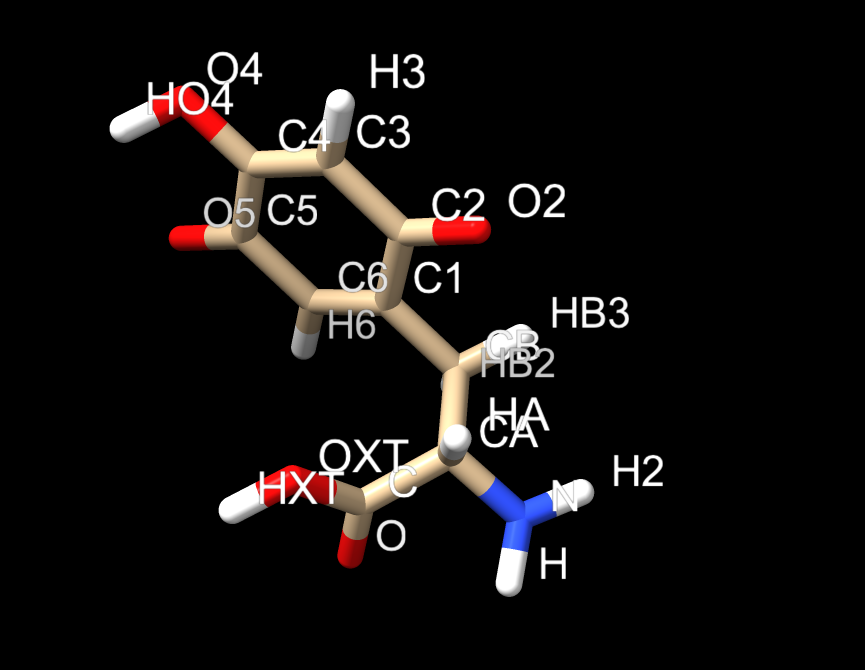
\includegraphics[width=0.5\linewidth]{TPQ_topo}
    \caption{Topology and atom names of the TPQ residue used in this calculation.}
    \label{fig:TPQ_topo}
\end{figure}
\begin{lstlisting}[language=Bash,caption={Prepgen command for TPQ}]
    prepgen -i tpq2.ac -o tpq.prepin -m tpq.mc -rn TPQ
\end{lstlisting}

By running that command a file containing the definition of the TPQ modified residue is generated into a prepi file. For now we have the residue library with the charges for the atoms in our modified amino acid; but the covalent parameters like bonds, angles and dihedrals are still needed.

To obtain those parameters the following command has to be run:

\begin{lstlisting}[language=Bash,caption={Parmchk2 command}]
    parmchk2 -i tpq.prepin -f prepi -o frcmod.tpq -s gaff2
\end{lstlisting}

By reading an ac file or a prep file it gives as an input an additional force field file (frcmod file) with the missing parameters. Every atom type can have one or more corresponding atom types for which force field parameters are changeable.
Having completed the TPQ parameterization, a similar process will be followed to parameterize NAG.
Initially the same first command used for TPQ with a change in the format output file (fo) is runned:

\begin{lstlisting}[language=Bash,caption={Antechamber for NAG}]
    antechamber -fi ccif -i NAG.cif -bk \
                NAG -fo prepi -o nag.prepin -c bcc -at amber
\end{lstlisting}

By this change in the command the output file directly is a prepi file. That change in this case provides an optimization because we are creating two less files since NAG is not a cofactor like TPQ that derives from a tyrosine that has been modified. As it is a carbohydrate, is not needed to create a mc file to transform it in an "amino-acid" like residue by the prepgen file. It is true, that all NAGs are linked to the protein by asparagine but the correctly way to address this linking to amber understand it, is by changing in our protein PDB file called DAO.pdb, look for the ASN (asparagine) that link NAGs to the protein and change that ASN for a NLN (N-linkage to ASN). It can be done manually one by one, or openning the file in Visual Studio Code, look for each ASN that has a N-linkage by simply doing a Control + F and replace them in the little window that appears for NLN. In this case the ASN to change are:

\begin{verbatim}
ASN A 126
ASN A 553
ASN B 768
ASN B 1195
\end{verbatim}

Continuing with NAG parameterization only lacks the frcmod file, that is obtained by using the prepi file as an input and the following command:

\begin{lstlisting}[language=Bash,caption={Parmchk2 command}]
    parmchk2 -i nag.prepin -f prepi -o frcmod.nag -s gaff2
\end{lstlisting}

Now the two files needed from TPQ and NAG are prepared.

After parameterizing each of the two non-standard residues of the protein, is needed to parameterize the carbohydrate, trehalose. This step was a little more complex because the CIF or PDB file of trehalose couldn't be found anywhere, then to obtain the file, the use of \href{https://www.cheminfo.org/Chemistry/Cheminformatics/FormatConverter/index.html}{Openbabel} was required.
First of all a file from drugbank in 3D mol format was downloaded. Then, that file was processed and transformed by Openbabel into a 3D coordinates PDB file. At the end we achieved a file that amber software could process by running the command pdb4amber.

To start with trehalose parameterization as in the previous cases first is used Antechamber on the input file:

\begin{lstlisting}[language=Bash,caption={Antechamber for trehalose}]
    antechamber -fi pdb -i tre.pdb -fo ac -o tre.ac -c bcc -at amber
\end{lstlisting}

Having the ac file, as well as previous parameterizations, still two files are required to be loaded in our tleap file, the prepi file and frcmod file. To get the prepi one, first thing to create is a main chain file for later use prepgen command. Considering that trehalose will be isolated, the main chain file only will have a line referring to the charge:

\begin{verbatim}
CHARGE 0.0
\end{verbatim}

With the main chain file created for the isolated trehalose, it is the time to use it as input the prepgen command

\begin{lstlisting}[language=Bash,caption={Trehalose prepgen}]
   prepgen -i tre.ac -o tre.prepin -m tre.mc -rn TRE
\end{lstlisting}

With that command now the prepi file generated is ready to be loaded in the tleap file. For the obtention of frcmod file, the prepi file is needed as an input file, so the command to use:

\begin{lstlisting}[language=Bash,caption={Trehalose parmchk2}]
   parmchk2 -i tre.prepin -f prepi -o frcmod.tre -a Y \ 
            -p $AMBERHOME/dat/leap/parm/parm10.dat
\end{lstlisting}

Since one of the objectives is to run five simulations with different number of trehalose molecules, five different files are needed, which for each one of them a different set of number of trehalose molecules where added by rotating and translocating them randomly with a Python program that was created based on Euler angles and randomization of the reorganization of \textit{N} molecules in space, with a separation between them at a minimum 3Å of distance.


\subsection{Tleap files}

Having the protein file and the parameterization files ready, they are need to be loaded into a tleap file along with other parameters. Tleap file, once it is run, it gives as an output the topology and coordinates files to use for simulations of the system created. Since different simulations will be performed, varying tleap files will be needed. Each variation of tleap file will be explained with each simulation in the following section.

\subsection{Amber simulations}

Typically every molecular simulation follows the same step by step workflow, probably adding, removing or changing steps depending on the simulation requirements.
In this project the workflow consisted in first of all obtaining the necessary PDB and CIF files for the protein, the components of it and the dissacharyde. After that we prepared the protein file and parameterize the components and the trehalose. Next to do was to generate different tleap files for each simulation. This procedure was performed in a very similar manner between each simulation(Table:\ref{tab:taulasimulations})


\begin{table}
\caption{Amber simulations}
\label{tab:taulasimulations}
\begin{tabular}{|c|}
    \hline
    \thead{Simulations to perform} 
    \\
    \hline
    Simulation of DAO in water system without ions, NAG ligand and trehalose
    \\
    \hline
    Simulation of DAO in water system with NAG, water, ions and trehalose (0,5M; 1M; 1,5M) 
    \\
    \hline
    Simulation of 1 trehalose molecule in water system
    \\
    \hline
    Simulation of 2 trehalose molecules in water system
    \\
    \hline
    Simulation of 5 trehalose molecules in water system
    \\
    \hline
    Simulation of 10 trehalose molecules in water system
    \\
    \hline
    Simulation of 25 trehalose molecules in water system
    \\
    \hline
  \end{tabular}
\end{table}




\subsubsection{DAO without NAG, ions or trehalose}
Before anything else, to extract NAG from DAO.pdb because is not going to be used in this simulation, running an easy command in the terminal, deletes every part of the document that contains NAG:

\begin{lstlisting}[language=Bash,caption={Trehalose prepgen}]
   grep -v NAG dao.pdb > daonag.pdb
\end{lstlisting}

For this simulation it is only needed to load the parameters of TPQ since we deleted NAG for this simulation. Ions were not added in this case. The tleap file for this simulation called tleap.in looked like this:

\begin{verbatim}
source leaprc.protein.ff19SB
source leaprc.water.opc
loadAmberPrep tpq.prepin
loadAmberParams frcmod.tpq
dao=loadpdb daonag.pdb
bond dao.132.SG dao.153.SG
bond dao.314.SG dao.340.SG
bond dao.774.SG dao.795.SG
bond dao.956.SG dao.982.SG
solvateOct dao OPCBOX 10.0
savepdb dao daowat.pdb
saveAmberParm dao dao.parm7 dao.rst7
quit
\end{verbatim}


The first two lines load the force fields we need for the simulation, both of the two following ones are the parameters files we created for TPQ. Next line loads our protein file of interest as a variable and gives it a name, in this occasion dao. Now we have reached the lines that by our explicit needs we specify that between those atoms there is a disulfide bond. This disulfide bonds are between CYX residues (a cysteine involved in a disulfide bridge).
Once every file needed was loaded it is time to solvate the system; that's what the solvateOct line is for. In this case we solvate the system in a truncated octahedral water box. Having the system completed we need to save a new PDB file of the system and save its topology (parm7) and coordinates(rst7) in two separate files. At the end of the file we must put simply quit to tell amber to shut off tleap. With the tleap file we have to run this command to execute it:


\begin{lstlisting}[language=Bash,caption={Trehalose prepgen}]
   tleap -f tleap.in
\end{lstlisting}

As a result of the run of that command we achieved three new files that would be used later for running the simulation. The new PDB file contains the system information of our protein inside a truncated octahedral water box (Figure \ref{fig:DAOWAT}) and the other two the initial coordinates and the topology of the system.

\begin{figure}[h]
    \centering
    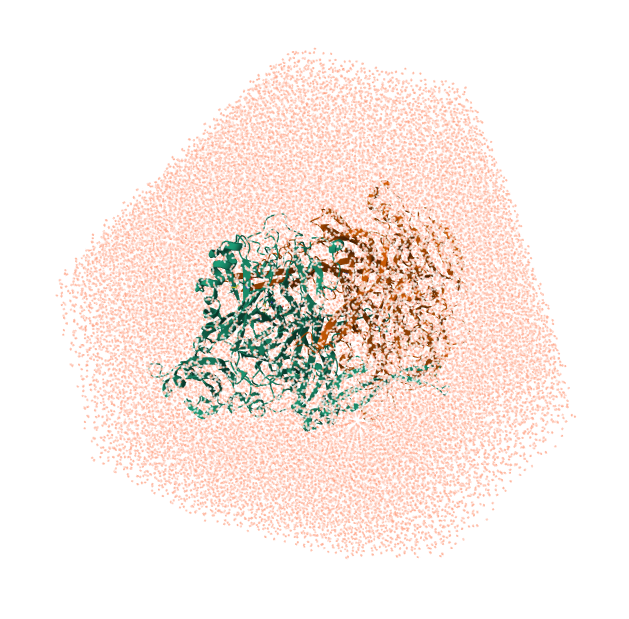
\includegraphics[width = 0.6\hsize]{./figures/DAOWAT.PDB}
    \caption{Starting coordinates and structure from the system of DAO without NAG into a truncated octahedral water box as a reference for simulation process (image obtained by 3D PDB viewer)}
    \label{fig:DAOWAT}
\end{figure}

Given that the simulation is runned in 3 steps: minimization, heating and production, we are going to create three different files to be used as inputs by amber.
The first file would be minimization file (called min.in) that must have certain parameters established as well as the other two. Minimization is a numerical process that begins with a higher energy initial structure and finds a minimum on the potential energy surface. In this particular minimization process of this simulation was like that:

\begin{verbatim}
  simple generalized Born minimization script
 &cntrl
   imin=1, ntb=1, maxcyc=100, ntpr=10, cut=8.0, ntmin=1,
 /
 
\end{verbatim}

Once the file is prepared it has to be executed from the terminal, in this case:

\begin{lstlisting}[language=Bash,caption={Trehalose prepgen}]
pmemd -O -i min.in -p dao.parm7 -c dao.rst7 -o min1.out -r min1.rst7
\end{lstlisting}

Running this command and using the min.in file as an input together with the coordinates and topology file from tleap, we get an output file that register the process of minimization and a restart file with the coordinates and velocities from the last step of minimization. After running minimization comes heating, as it name suggests consists of the progressive increase of temperature of the system very slowly until it reaches the desired temperature.
Heating file called heat.in had this structure:


\begin{verbatim}
Explicit
 &cntrl
   imin=0, irest=0, ntx=1,
   ntpr=1000, ntwx=1000, nstlim=100000,
   dt=0.002, ntt=3, tempi=0,
   temp0=300, gamma_ln=5.0, ig=-1,
   ntp=0, ntc=2, ntf=2, cut=8.0,
   ntb=1, igb=0, ioutfm=1, nmropt=1,
 /
 &wt
   TYPE='TEMP0', ISTEP1=1, ISTEP2=100000,
   VALUE1=10.0, VALUE2=300.0,
 /
 &wt TYPE='END' 
 /

\end{verbatim}

As in minimization process, the file it has to be executed by a command from the terminal:

\begin{lstlisting}[language=Bash,caption={Heating run}]
pmemd -O -i heat.in -p dao.parm7 -c min1.rst7 -o heat.mdout \
       -x heat.nc -r heat.rst7
\end{lstlisting}

Using the heat.in as an input file along with the coordinates file from minimization and the topology file, the command returns just as in the previous step an output file with the heating register and a restart file with coordinates and velocities from heating; but in addition it gives an extra file, the heat.nc file which is the one that saves the trajectory of the system during the heating process.
Lastly we have to run the largest process in molecular dynamics simulation which is the production. As in the previous processes, we have to create a new file to run this process, for this production the file was named md.in:


\begin{verbatim}
Explicit md
 &cntrl
   imin=0, irest=1, ntx=5, ntt=3,
   ntpr=1000, ntwx=1000, ntwr=1000, nstlim=500000000,
   dt=0.002, ntt=3, tempi=300,
   temp0=300, gamma_ln=2.0, ig=-1,
   ntp=1, ntc=2, ntf=2, cut=8.0,
   ntb=2, igb=0, ioutfm=1,
 /

\end{verbatim}

Repeating the cycle like in the previous two steps of simulation, to use the md.in file with the heating restart file, a code to run in the terminal is needed:

\begin{lstlisting}[language=Bash,caption={Heating run}]
    pmemd -O -i md.in -p dao.parm7 -c heat.rst7 -o md1.mdout \
       -x md1.nc -r md1.rst7    
\end{lstlisting}


Given that this command would take a lot of time to be completed since uses local CPU, the GPU from a supercomputer was required. Logging into a supercomputer by ssh connection, all the files were copied there to work on; in addition a new bash file to run in the supercomputer was created (md.batch) to run the process:

\begin{verbatim}
#!/bin/bash
#SBATCH -J mddao
#SBATCH -e %J.%j.err
#SBATCH -o %J.%j.out
#SBATCH -p gpu
#SBATCH -n 1
#SBATCH -t 0-24:00
module load apps/amber/22
##
#  Modify the input and output files!
cp -r ${SLURM_SUBMIT_DIR}/{*.in,*.parm7,*.rst7} $SCRATCH
cd $SCRATCH
echo $(SCRATCH)
echo $(SLURM_SUBMIT_DIR)
echo $SCRATCH
ls
pwd
pmemd.cuda -O -i md.in -p dao.parm7 -c heat.rst7 -o \
md1.mdout -x md1.nc -r md1.rst7
cp ./*.out ${SLURM_SUBMIT_DIR}
\end{verbatim}

To run this new file in the supercomputer, from the terminal logged by ssh (secure shell) connection we have to run the following command:

\begin{lstlisting}[language=Bash,caption={Submitting job into supercomputer}]
    sbatch md.batch
\end{lstlisting}

The outputs of this command are the same that in heating step, a registration, a trajectory and a restart output files. Due to the large time it takes to run a production process of a simulation, normally it takes more than one run; in this production 15 runs were needed because the calculations took 24 hours each to be completed. Since the same production process was divided in 15 runs, each time a run finished, its restart output file was used in the following run as an input coordinates file so the process wouldn't be lost.


\subsubsection{Trehalose simulations}

Before preparing a simulation containing the protein and trehalose in a water system, a first verification of the stability of trehalose will be done. For the stability testing, five different simulations with a different number of trehalose molecules in each of them.


\begin{figure}[h]
    \centering
    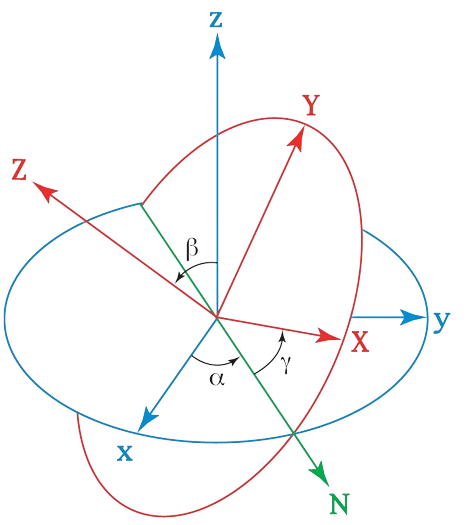
\includegraphics[width = 0.4\hsize]{./figures/euler}
    \caption{Two orthogonal coordinates system where Euler angles are shown }
    \label{fig:euler}
\end{figure}


\begin{figure}[h]
    \centering
    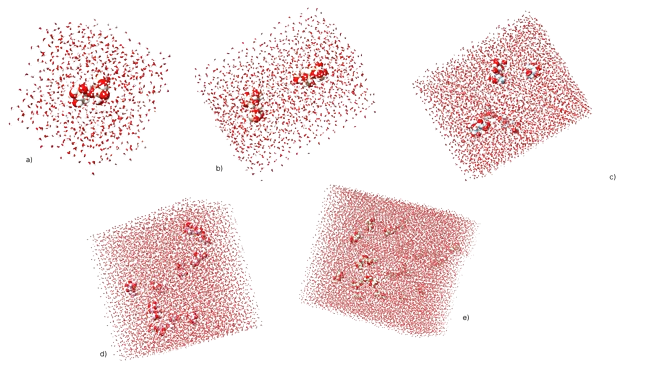
\includegraphics[width = 1\hsize]{./figures/trewat}
    \caption{Different cubic water box systems with different number of trehalose molecules inside: a) 1 trehalose molecule, b) 2 trehalose molecules, c) 5 trehalose molecules d) 10 trehalose molecules, e) 25 trehalose molecules. Images got with ChimeraX}
    \label{fig:trewat}
\end{figure}

As mentioned earlier, to generate five different files to be used in each simulation, a Python program was created. The program called "addtobox" was based in different parameters. First of all, it used as an input file the trehalose ac file obtained in the preparation file process which includes the partial charges. The orientation of one typically mobile orthogonal axis reference system with respect to another normally fixed orthogonal axis reference system is specified using a set of three angular coordinates known as Euler angles (Figure \ref{fig:euler}), so an array of randomized Euler rotation angles is created to use later. In parallel a translation vector is generated. The next thing was to read the ac file coordinates and extract them into an array which then for every molecule number desired would be add in different chains into a new PDB file. Having a file with the coordinates copied according to the number of desired molecules we apply the translation vector and the Euler array generating new rotated and translated coordinates from the original.

The Python program was runned five times generating five different files with different number of molecules (Figure \ref{fig:trewat}).

Once the files were generated they were processed like the protein PDB file. Since we already have parameterization files for trehalose it is not necessary to create new ones, the only difference for each simulation is the tleap file as the other ones can be shared. The difference resides in the PDB file that is load in the tleap, as in the example below, the loadpdb would change for every tleap:

\begin{verbatim}
source leaprc.protein.ff19SB
source leaprc.water.opc
source leaprc.GLYCAM_06j-1
set default PBRadii mbondi3
loadAmberPrep tre.prepin
loadAmberParams frcmod.tre
tre=loadpdb tre-copy.pdb
solvateBox tre OPCBOX 10.0
savepdb tre tre1hwat.pdb
saveAmberParm tre tre1.parm7 tre1.rst7
quit
\end{verbatim}


For the shared files we have the minimization, heating and production files. Although these files are shared, we have to change in the command it executes the different topology and coordinates files for each one of the simulation.

The minimization file (min.in) used to minimize the system was:

\begin{verbatim}
      simple generalized Born minimization script
 &cntrl
   imin=1, ntb=1, maxcyc=100, ntpr=10, cut=8.0, ntmin=1,
 /

\end{verbatim}

As can be seen, each of the files differ one of each other in some of the parameters, the value of those, the quantity... This is because each step of the simulation requires different parameters to be assigned. Not only the parameters between different steps of simulation are different, but for every simulation a new system of files is needed. The structure of this heating file is this way:

\begin{verbatim}
    Explicit
 &cntrl
   imin=0, irest=0, ntx=1,
   ntpr=1, ntwx=1000, nstlim=2000,
   dt=0.002, ntt=3, tempi=0,
   temp0=300, gamma_ln=5.0, ig=-1,
   ntp=0, ntc=2, ntf=2, cut=8,
   ntb=1, igb=0, ioutfm=1, nmropt=1,
 /
 &wt
   TYPE='TEMP0', ISTEP1=1, ISTEP2=100000,
   VALUE1=10.0, VALUE2=300.0,
 /
 &wt TYPE='END' 
 /

\end{verbatim}

And the production file to run in supercomputer:

\begin{verbatim}
    #!/bin/bash
#SBATCH -J md1tre
#SBATCH -e %J.%j.err
#SBATCH -o %J.%j.out
#SBATCH -p gpu
#SBATCH -n 1
#SBATCH -t 0-12:00
module load apps/amber/22
##
#  Modify the input and output files!
cp -r ${SLURM_SUBMIT_DIR}/{*.in,*.parm7,*.rst7} $SCRATCH
cd $SCRATCH
echo $(SCRATCH)
echo $(SLURM_SUBMIT_DIR)
echo $SCRATCH
ls
pwd
pmemd.cuda -O -i md.in -p tre1.parm7 -c \
tre1heat.rst7 -o tre1md.mdout -x tre1md.nc -r tre1md.rst7
cp ./*.out ${SLURM_SUBMIT_DIR}

\end{verbatim}


\subsubsection{DAO with NAG and trehalose simulation}

The last simulation to be prepared is the one that contains the protein, all of its cofactors, the carbohydrate, ions and the cubic water box completing the system.

It follows basically the same preparation that was used for the first simulation with some changes in it. The first thing that is needed is the PDB file of DAO 
(code 1KSI from RCSB) prepared for Amber by running the pdb4amber command, but in this case the lines containing NAG are needed so they will not be erased. This simulation, unlike the one consisting of DAO without NAG, requires the addition of new command lines in its tleap file:

\begin{verbatim}
source leaprc.protein.ff14SB
source leaprc.water.opc
source leaprc.GLYCAM_06j-1
loadAmberPrep tpq.prepin
loadAmberPrep nag.prepin
loadAmberParams frcmod.tpq
loadAmberParams frcmod.nag
dao= loadpdb dao.pdb
bond dao.132.SG dao.153.SG
bond dao.314.SG dao.340.SG
bond dao.774.SG dao.795.SG
bond dao.956.SG dao.982.SG
bond dao.1287.C1 dao.768.ND2
bond dao.1287.O4 dao.1288.C1
bond dao.1292.C1 dao.1195.ND2
bond dao.126.ND2 dao.1285.C1
bond dao.1285.O4 dao.1286.C1
bond dao.553.ND2 dao.1289.C1
addions dao NA 0
solvateBox dao OPCBOX 10.0
savepdb dao daowat.pdb
saveAmberParm dao dao.parm7 dao.rst7
quit

\end{verbatim}

As it can be seen in the tleap file, a new force field has been added (GLYCAM06-j) which is the one for carbohydrates as NAGs and trehalose. Also new bonds have been specified that represent the bonds between NAG-ASN or NAG-NAG. The last two differences comparing to the first simulation is the addition of Sodium (Na) ions to address a charge of 0 in the global system, and at last the solvation of the system into a water cubic box.

Running the file several errors have been shown. The first error shown was that some NAGs did not have an atom type, which should not be the case because the parameterization files were loaded. Looking at the error carefully shows that only the NAGs are linked between them and to an ASN (ASN-NAG-NAG) are the ones presenting an error.

In a first attempt to correct the error, the assembly of a new residue was tried. It consisted of hooking up the sequences of the ASN and NAGs that were linked between them into a new file and process it as it was a PDB or CIF file downloaded from the web. This try was to no avail.

Another attempt to solve the error consisted in changing the residue name from each of those NAGs into 0YB or 4YB (as GLYCAM section in the Amber manual it is shown), being the 0YB the NAG connected to ASN and the 4YB the NAG linked to the other NAG. At first it seemed that the error was corrected, but it was not and another error appeared.

At the end it was decided to erase those NAG and solvate the system anyway and after that, trehalose was added in a concentration of 0.5M. The addition of trehalose was done into the output file from solvation and considering the volume of it to know how many molecules of trehalose were needed to add. To calculate the number of trehalose molecules needed, first is necessary to know the total volume of the system, that was 1611694.133 ų. From there the calculations are:

\[
V = 1,611,694.133 \, \text{\AA}^3 \cdot \frac{10^{-27} \, \mathrm{litres}}{\text{\AA}^3}= 1.611,694,133 \cdot 10^{-21} \, \mathrm{litres}
\]
\[
0.5\, \mathrm{M} \cdot 1.611,694,133 \cdot 10^{-21} \, \mathrm{litres} = 8.058,470,665 \cdot 10^{-22}\,  \mathrm{moles}
\]

\[
8.058,470,665 \cdot 10^{-22}\,  \mathrm{moles} \cdot 6.022 \cdot 10^{23} = 485 \, \mathrm{molecules}
\]
After this simple calculations and given as a result the needed number of trehalose molecules to add, we use the command called AddToBox as it is shown:

\begin{lstlisting}[language=Bash,caption={AddToBox command}]
    $AMBERHOME/bin/AddToBox -c daowat.pdb -a tre.pdb -na \
    485 -o daotrewat.pdb -P 20712 -RP 2.0 -RW 3.0 -G 0.2
\end{lstlisting}

The result of this command is a system with the protein, almost all of its cofactors except for the NAG polymers, the carbohydrate, ions and water (Figure \ref{fig:daotrewat}).

\begin{figure}[h]
    \centering
    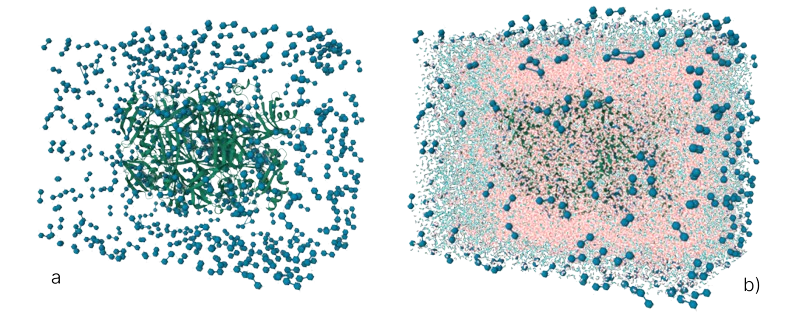
\includegraphics[width = \linewidth]{./figures/daotrewat}
    \caption{The system composed by the protein, its cofactors, water, carbohydrate and ions: \textbf{a)} water molecules not visible, only trehalose (blue molecules) and the protein; \textbf{b)} all the system visible}
    \label{fig:daotrewat}
\end{figure}

\subsection{Results visualization}
As the results we transfer from the supercomputer to our local machine are data files with numbers on it, the processing of those files is essential. From the \texttt{*.mdout} files, we get a lot of information, but it cannot be interpreted or plotted. In order to solve this issue, a Python program called \texttt{dataframes.py} was created to perform the function of structuring the data. At the same time another program called \texttt{graphs.py} was created to generate plots as desired like choosing more than one variable to compare or simply the values from only one variable against another one. The \texttt{*.mdout} files are not the only type of file that we get as an output from a simulation, but also trajectory files. These are more complicated to graph because they format are binary, so other program is needed. To initialize the process of graphing these results, first is needed to call cpptraj (once installed) from the terminal in the computer by writing cpptraj on it.
For each result the same process was followed, so to take as an example, only one will be explained. Once cpptraj is runned it will appear:

\begin{verbatim}
    CPPTRAJ: Trajectory Analysis. V6.18.1 (AmberTools)
    ___  ___  ___  ___
     | \/ | \/ | \/ | 
    _|_/\_|_/\_|_/\_|_

| Date/time: 06/02/24 19:32:04
| Available memory: 397.255 MB

	Loading previous history from log 'cpptraj.log'

\end{verbatim}

Next thing to do was to load topology and trajectory files:

\begin{lstlisting}[language=Bash,caption={Loading topology file}]
    parm file
\end{lstlisting}
\begin{lstlisting}[language=Bash,caption={Loading trajectory file}]
    trajin file
\end{lstlisting}

With the two or more needed files are loaded by a specific command that can be found in \href{https://ambermd.org/tutorials/analysis/tutorial1/index.php}{AmberTutorials}:


\begin{lstlisting}[language=Bash,caption={RMSD command}]
    rms ToFirst :1-13&!@H= first out rmsdtre1.agr mass
\end{lstlisting}

With the cpptraj prepared, the only thing left is to run it by typing the word "run". Once is processed the only thing to do is to visualize the results with xmgrace or other visualization tool:

\begin{lstlisting}[language=Bash,caption={Visualization}]
    xmgrace rmsdtre1.agr
\end{lstlisting}

This process is repeated for each of the simulations with the amount of trajectory files one wants. 

	

\end{document}